\documentclass[titlepage,11pt]{article}
\usepackage[utf8]{inputenc}
\usepackage{fullpage}
\usepackage{indentfirst}
\usepackage[per-mode=symbol]{siunitx}
\usepackage{listings}
\usepackage{graphicx}
\usepackage{color}
\usepackage{amsmath}
\usepackage{array}
\usepackage[hidelinks]{hyperref}
\usepackage[format=plain,font=it]{caption}
\usepackage{subcaption}
\usepackage{standalone}
\usepackage[nottoc]{tocbibind}
\usepackage{scrextend}
\usepackage[margin=1in]{geometry}
\usepackage{lstautodedent}
\usepackage[super]{nth}
\usepackage{todonotes}
\usepackage[noabbrev,capitalize,nameinlink]{cleveref}

\definecolor{dkgreen}{rgb}{0,0.6,0}
\definecolor{gray}{rgb}{0.5,0.5,0.5}
\definecolor{mauve}{rgb}{0.58,0,0.82}

\lstset{frame=tb,
  language=Java,
  aboveskip=3mm,
  belowskip=3mm,
  showstringspaces=false,
  columns=flexible,
  basicstyle={\small\ttfamily},
  keywordstyle=\color{blue},
  commentstyle=\color{dkgreen},
  stringstyle=\color{mauve},
  breaklines=true,
  breakatwhitespace=true,
  tabsize=3,
  basicstyle=\scriptsize\tt,
  autodedent,
  numbers=left,
  numberstyle=\tiny\color{gray},
  xleftmargin=2.5em,
  frame=single,
  framexleftmargin=2em
}

\def\equationautorefname~#1\null{%
  Equation~(#1)\null
}

\def\sectionautorefname~#1\null{%
  Section~#1\null
}

\def\subsectionautorefname~#1\null{%
  Subsection~#1\null
}

\def\arraystretch{1.3}%  1 is the default, change whatever you need

% Custom commands
\newcommand{\ar}[1]{\autoref{#1}}
\newcommand\numberthis{\addtocounter{equation}{1}\tag{\theequation}}
\newcolumntype{P}[1]{>{\centering\arraybackslash}p{#1}}
\newcommand{\code}[1]{\texttt{#1}}
\newcommand{\specialcell}[2][c]{%
	\begin{tabular}[#1]{@{}c@{}}#2\end{tabular}}

\title
{
	\uppercase{Prometheus AI} \\
	\large Phase 2
}
\author % (optional, for multiple authors)
{
	Sean Stappas \\ 
	260639512 \\
	\\ 
	ECSE-499: Honours Thesis II \\
	\\
	\small Supervised by: Prof. Joseph Vybihal
}
\date{December \nth{7}, 2017}

\begin{document}
	
\sloppy

\maketitle

\section*{Abstract}
% The abstract is an executive summary of your project/thesis. It should provide an overview of your project/thesis by addressing the following questions. a. What is the motivation for the project/thesis? b. What are the goals of the project/thesis? c. What was achieved this semester? d. What methods were used to make those achievements? The abstract should be between 200 and 250 words long.
Prometheus AI is a model of the human brain with the goal of controlling and coordinating multiple robots in different environments. This could be useful in environments hazardous for humans, such as in the aftermath of a nuclear power disaster, or in outer space. The model consists of four layers: the Neural Network (NN), the Knowledge Node Network (KNN), the Expert System (ES), and the Meta Reasoner (META). The NN classifies the signals coming from the robots' sensors and sends formatted tags to the KNN. The KNN represents memory and can initiate cascaded activation of memories in the form of tags, which are passed on to the ES. The ES is a simple logic reasoner and provides recommendations for actions to the META. The META represents high-level thinking and makes an intelligent decision for the robots. The tasks for this thesis were to implement the KNN and ES layers in Java and to supervise work done by undergraduate students on Prometheus. This was achieved using specific design criteria and extensive feedback from the project supervisor, Prof. Vybihal. Personal design criteria included using object-oriented programming principles, optimizing the system for speed and space efficiency, and maximizing code readability and testability. Continuous integration tests were created with TestNG and TravisCI and extensive documentation was written in Javadoc.

\section*{Acknowledgments}
% If applicable, you may acknowledge people here who contributed to the project in some way but are not listed on the title page. (For example, if you received advice, data, or supervision from graduate students or others.)
Under my supervision, several undergraduate students worked on the Prometheus layers in Prof. Vybihal's lab. Over the summer, Isaac Sultan and Si Yi Li made contributions to the ES and KNN layers, respectively. This semester, Mohammad Owais Kerney and Michael Ding showed interest in the NN and META layers, respectively.

\clearpage
\tableofcontents

\listoffigures
\listoftables
\lstlistoflistings
\clearpage

\twocolumn

\section*{Abbreviations}
% List of abbreviations and/or notation used in the report.

The following abbreviations will be used throughout the report:

\begin{table}[!htb]
	\centering
	\caption{Abbreviations in Prometheus.}
	\begin{tabular}{r | l}
		\textbf{Symbol} & \textbf{Meaning} \\ \hline
		NN & Neural Network \\
		KNN & Knowledge Node Network \\
		KN & Knowledge Node \\
		ES & Expert System \\
		META & Meta Reasoner \\
		OOP & Object-Oriented Programming
	\end{tabular}
	\label{table:abbrevations}
\end{table}

\section{Introduction} \label{sec:intro}
% In this section you should introduce (at a high level) the overall theme of the project, and state clearly what are the goals you are trying to achieve.  This section should also clearly convey why this project is important, what is the potential impact (applications, etc).

The goal of the Prometheus project is to create an artificial intelligence system to control and coordinate multiple robots. All the thinking and decision-making is done by Prometheus, which collects data from all the robots' sensors.

Applications for this type of system include robots in hazardous environments, such as in outer space (Mars, Moon, etc.), in nuclear plants after a disaster, and in military zones.  The system could ideally learn from this data in a given environment and apply its learning to new environments.

The system is loosely inspired from the structure of the human brain, and is composed of the following four layers \cite{vybihal-model}: the Neural Network (NN), the Knowledge Node Network (KNN), the Expert System (ES), and the Meta Reasoner (META), which can be seen in \autoref{model}.

\begin{figure*}[!htb]
	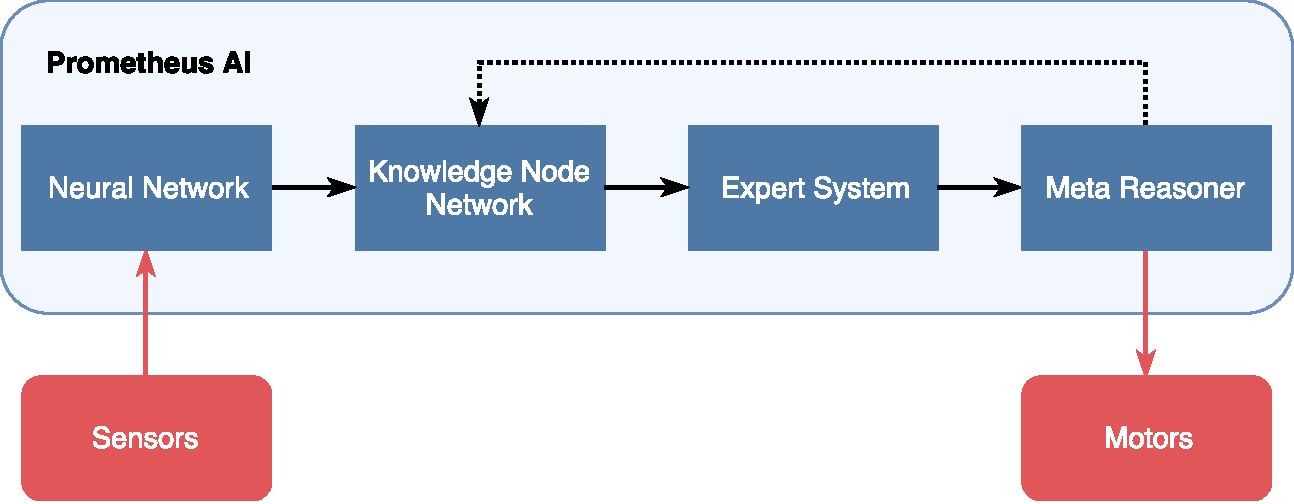
\includegraphics[width=\textwidth]{figures/ai_model.pdf}
	\caption[Prometheus AI model.]{Prometheus AI model. Blue represents Prometheus and green represents the robots.}
	\label{model}
\end{figure*}

The theory needed to understand these four layers will be given in \autoref{sec:background}. The assigned task will then be described in \autoref{sec:problem}. Design criteria will be discussed in \autoref{sec:design}. The description of the work done this semester can be found in \autoref{sec:implementation}, and the results and tests will be discussed in \autoref{sec:results}. Finally, the possible future impact of this project on society and the environment will be explored in \autoref{sec:impact}.

The scope of this thesis is primarily to implement the KNN and ES in Prometheus. Therefore, more detail will be given for these layers.

\section{Background} \label{sec:background}
% In this section you should summarize the theory and background that you had to learn, and that you believe are necessary for the reader to understand the rest of the report.
This section draws heavily from the background discussed in the previous report \cite{stappas}.

\subsection{Neural Network}

The NN layer consists of a network of neurons with a structure similar to neurons in the human brain. It is the interface between the robots' sensors and the rest of the AI system.

The robots in Prof. Vybihal's lab are equipped with two types of sensors: camera and ultrasonic. The ultrasonic sensor can measure distance between the robot and nearby objects, and the camera can take images of what the robot is facing.
%The robots have a fixed front-facing camera. Each robot may have multiple fixed ultrasonic sensors pointing in different directions, or a single rotating ultrasonic sensor that sweeps the area in front of the robot. 

The NN gathers raw sensor data and will build an abstract view of the robot's surrounding environment. For each camera image, it will achieve two main goals:

\begin{enumerate}
	\item Classify objects observed in the image.
	\item Localize objects in the image.
\end{enumerate}

Ultimately, the classification and localization of objects will produce abstract informational tags, which will be passed on to the KNN. These tags can therefore be characteristics of objects in the world, such as distance. The tags can also have associated confidence confidence values produced by the NN, which can be converted to belief within the KNN.

\subsection{Knowledge Node Network}

The KNN layer represents memory in the human brain. It takes in the tags provided by the NN and outputs tags based on its knowledge of the environment. The KNN is based around interconnected Knowledge Nodes (KNs), which are abstract structures representing memories and their connections to other memories. A simple model of a Knowledge Node (KN) can be seen in \ar{kn}.

\begin{figure}[!htb]
	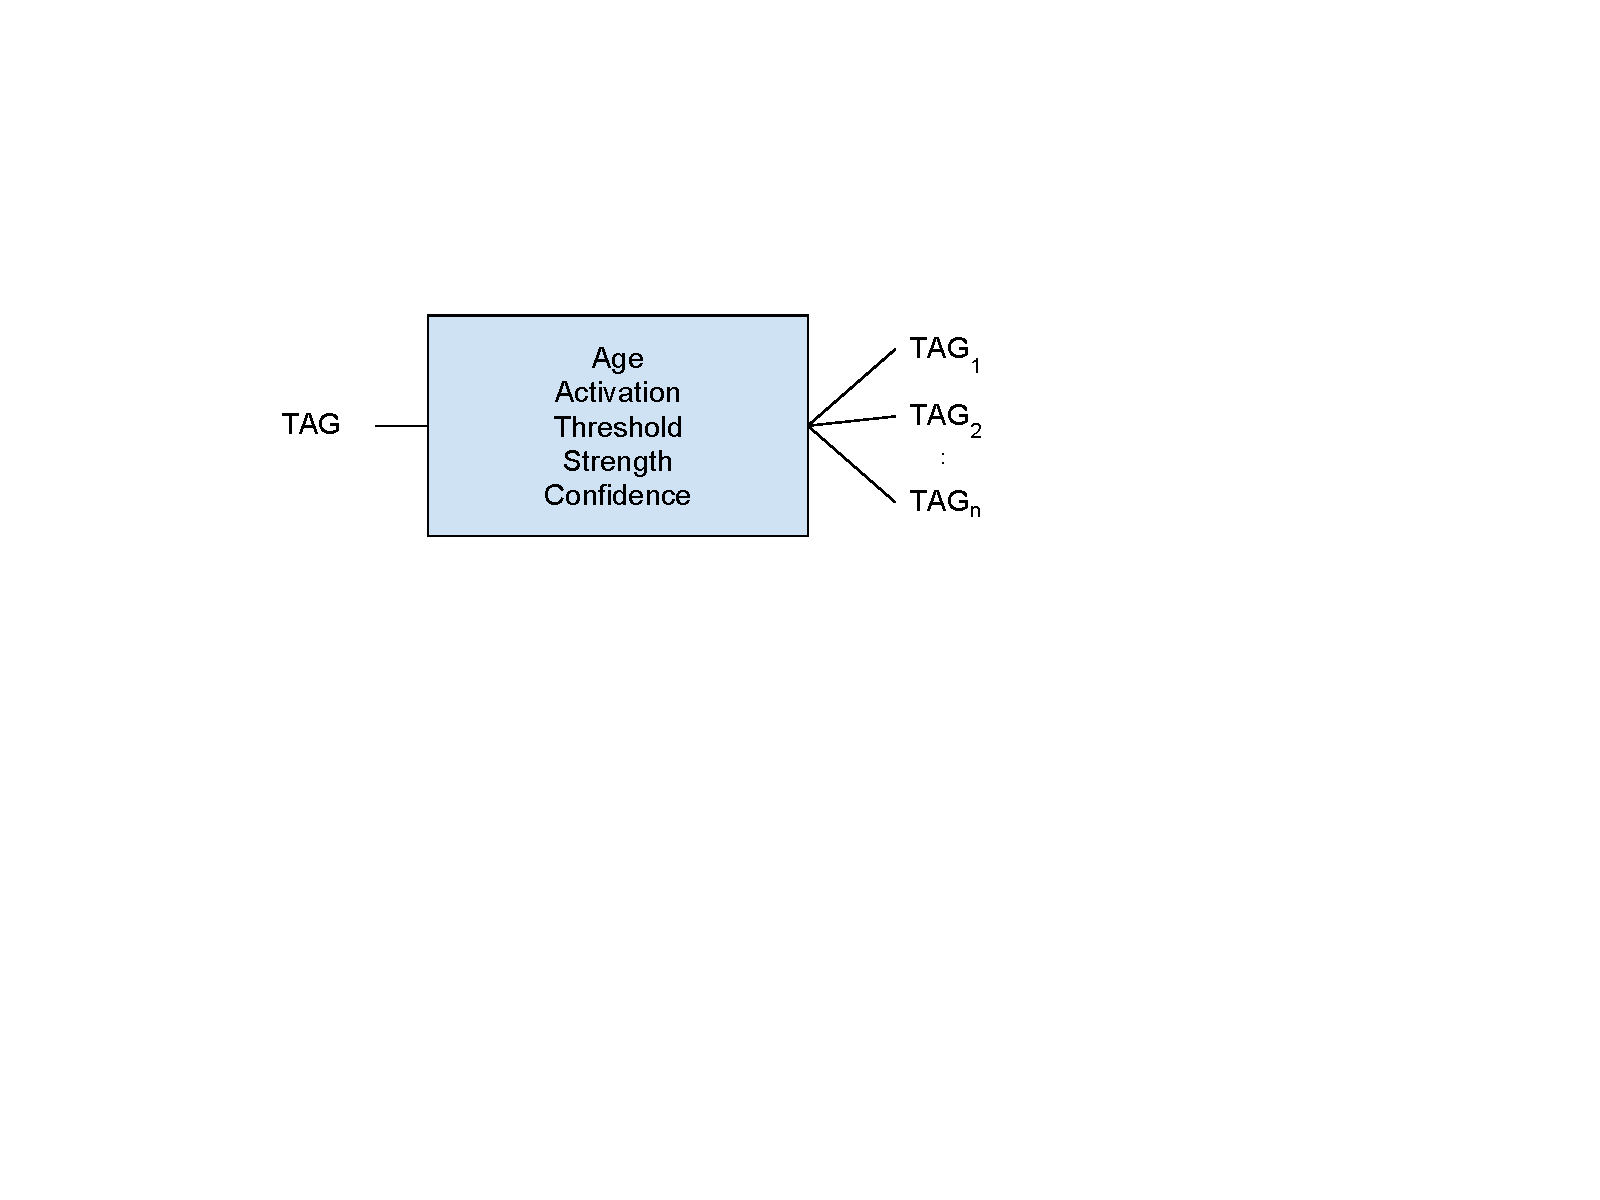
\includegraphics[width=\columnwidth]{figures/kn.pdf}
	\caption[High-level model of the Knowledge Node of the KNN.]
	{High-level model of the Knowledge Node (KN) of the KNN \cite{vybihal-knowledge}.}
	\label{kn}
\end{figure}

KNs have an input tag representing some information, and output tags representing information related to the input tag. When a KN is stimulated it becomes ``excited''. Tags in the KNN can become ``active'', meaning the associated KN is stimulated beyond a threshold. We say that the associated KN ``fires'' in this case. For example, if the NN determines that it observes a ball and passes that information on to the KNN, then a ``ball'' tag may become active in the KNN. This would excite the KN with input tag ``ball''. If that KN fires, other tags related to that observation can become active. For example, tags representing ball characteristics such as ``round object'' may become active. This tag in turn may be connected to another KN, potentially causing more activation.

There are different ways that KN excitation could be implemented. With simple linear activation, excitation would increment the node's activation parameter, which initially starts at 0. If $activation \geq threshold$, the KN fires, causing the activation of the output tags. This description corresponds to forwards thinking. The activation can also be achieved using a sigmoid function, which is more representative of neurons in the brain \cite{neuro}.


There is a strength value associated with every KN which represents how much weight an activation has and therefore how quickly that node will fire. A simple implementation of strength would be as a constant coefficient multiplying the activation parameter. So, instead of checking when the activation is greater than the threshold, one would check if $activation * strength \geq threshold$, where the strength is positive. The strength value could be 0 however, which effectively shuts off the KN. Another way of implementing strength is to check $activation + strength \geq threshold$. In this case, strength can be negative and make the KN fire later than normal.

Strength can be seen as the firing predisposition of neurons in the brain as a result of learning \cite{vybihal-knowledge}. Indeed, learning can increase the synaptic strength between neurons and cause early  firing of those neurons \cite{hebb}. For example, a person who has had a bad experience with spiders would fire their fear response upon seeing a spider more quickly than one without that fear.

Every KN can have a belief value associated with it, representing how certain the KNN is that the input tag is true. In this case, the belief value would be stored within the KN itself. These belief values can come from the NN, since a neural network can associate confidence values with its classifications of objects \cite{mitchell1997machine}. When initiating a think cycle, the belief values at each stage can be multiplied with each other to produce a new confidence value, making the KNN less certain of a memory as it searches through its tree of KNs. This represents how belief changes when thinking. Indeed, some memories in the brain require a great deal of thinking to reach and, as such, can be less certain than other memories. This can lead to the recollection of false memories \cite{falsememories}.

Note that the activation of a KN and the belief value associated with it are two different concepts. Indeed, a KN may be fired even if the KNN knows that it is false. This can represent an agent ``lying'' to itself or repeating a thought process it knows to be false. This is known as ``self-deception'' in humans and it has been argued that this can be used for positive mental health \cite{taylor1989positive}.

Age represents how long it has been since a KN has been excited. The idea is that, after a KN has aged a certain amount of time, that node will be discarded, similarly to how old memories are discarded in the brain \cite{aging}. The intuitive implementation of aging is to constantly increment some age value associated with every KN, and discard nodes whose age is greater than some threshold. The age would be reset to 0 when the node is excited. This would however be unnecessarily computationally intensive, requiring some kind of constant updating of every single node. A more efficient way of doing it would be to save a timestamp for every KN when it is excited, and if the KNN attempts to excite a KN whose previous timestamp value is too far into the past, that node is instead deleted.
\todo{Move some of this to implementation?}

Searching in the KNN represents an activation routine, which activates tags and potentially fires KNs. The KNN has four ways of searching: direct, forward, backward, and lambda. Thinking in the KNN is a related concept to searching. Whereas in search input tags are provided to guide the KNN, in thinking, the KNN uses its currently active tags to activate further tags. In this way, thinking is a special case of searching, where the input tags of the search are the active tags in the KNN. The KNN has three ways of thinking: forward, backward, and lambda. The version of searching or thinking to be done by the KNN is chosen by the META. 

Direct searching is a simple lookup of the desired Tag and excitation of the associated KN. This represents the simplest form of thinking in the KNN and can be seen in \cref{fig:direct_search}.

\begin{figure}[!htb]
	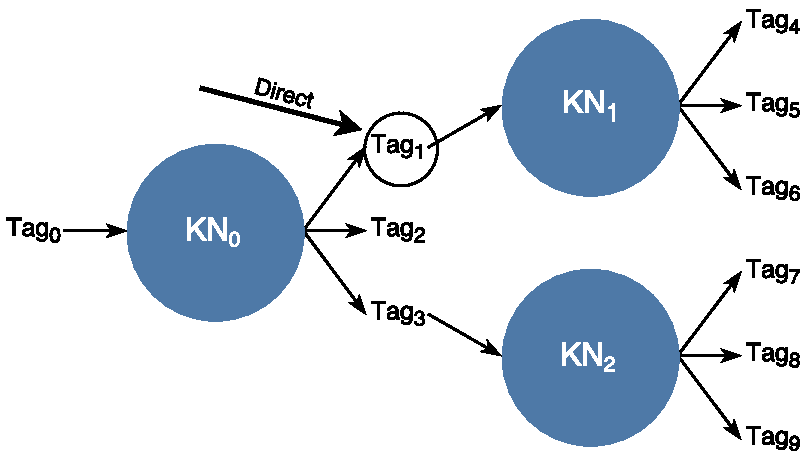
\includegraphics[width=\columnwidth]{figures/direct_search.pdf}
	\caption{Direct search in the KNN.}
	\label{fig:direct_search}
\end{figure}

Forward thinking is depicted in \autoref{think_forwards}. Firing a KN can cause forward activation of more KNs, hence the ``forwards'' naming.

\begin{figure}[!htb]
	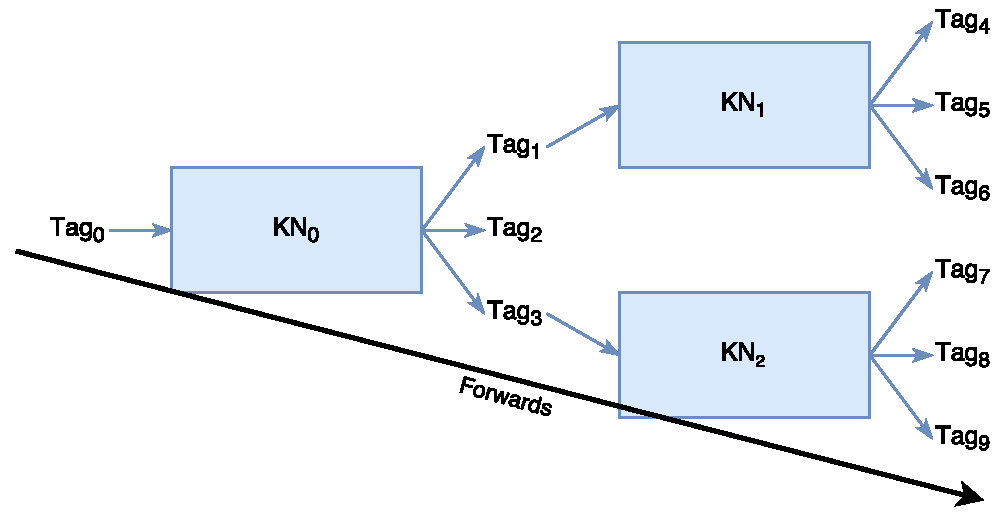
\includegraphics[width=\columnwidth]{figures/forwards_thinking.pdf}
	\caption{Thinking forwards in the KNN.}
	\label{think_forwards}
\end{figure}

Thinking backward starts at the output tags of KNs, and works backwards, as can seen in \autoref{think_backwards}. In its simplest form, it checks output tags of KNs and, if all of them are active, the input tag must be active as well, so that KN is fired.

\begin{figure}[!htb]
	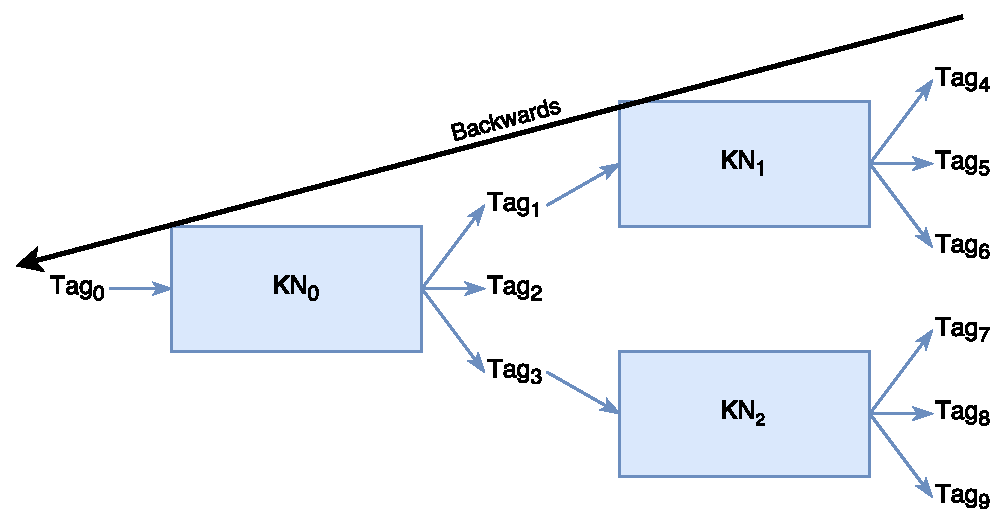
\includegraphics[width=\columnwidth]{figures/backwards_thinking.pdf}
	\caption{Thinking backwards in the KNN.}
	\label{think_backwards}
\end{figure}

This type of thinking can be more difficult to implement than forwards thinking, since one must decide what percentage of active output tags of a KN corresponds to an active input tag. For instance, should a KN fire when 100\% of its output nodes are active, or when 75\% are active? This relates to the belief with which the KNN believes the tag associated with that node to be true. As a concrete example, if you observe an object that has four wheels, seats, and a steering wheel, how confident are you that that object is a car? Realistically, humans will often classify what they observe with some uncertainty \cite{uncertainty} and this can be represented with backwards thinking. This type of thinking occurs constantly in the background in humans \cite{vybihal-knowledge}, and this is something to keep in mind during implementation.

Lambda thinking uses a combination of forwards and backwards, and can be seen in \autoref{think_lambda}. It is called ``lambda'' thinking because the shape of the thinking trajectory matches a Greek uppercase lambda ($\Lambda$). It first looks at output tags of KNs and propagates activation backwards, similar to backwards thinking. After a certain amount of nodes are fired, it will then start activating forwards, similar to thinking forwards. An interesting question is how far backwards should lambda thinking go before starting to cascade forwards? This relates to how general one wants to explore before searching for a more specific value.

\begin{figure}[!htb]
	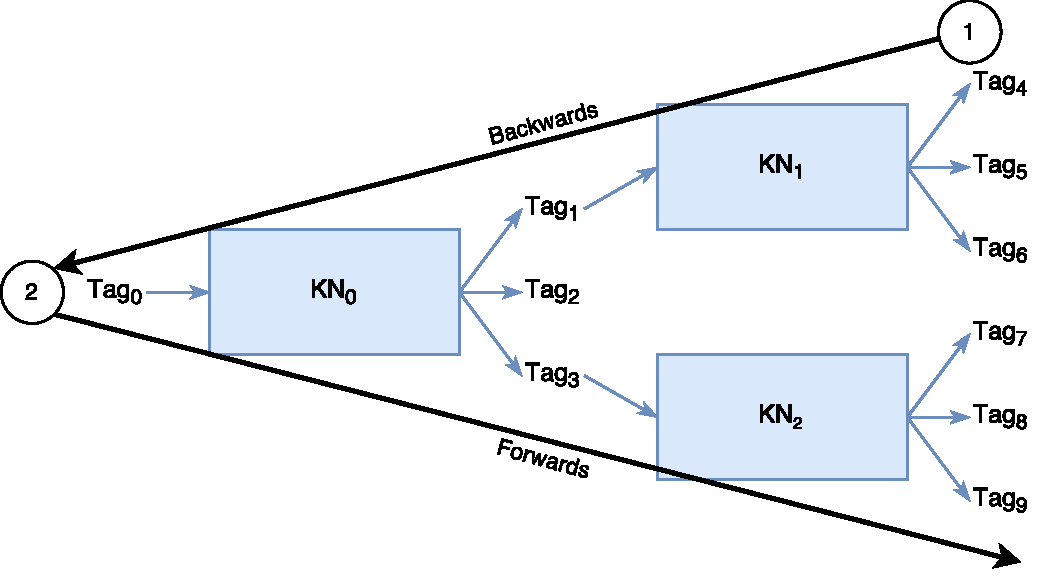
\includegraphics[width=\columnwidth]{figures/lambda_thinking.pdf}
	\caption{Lambda thinking in the KNN.}
	\label{think_lambda}
\end{figure}

This type of thinking occurs in humans when using analogical reasoning to find a memory \cite{vybihal-lambda}. In essence, when a person wants to locate a memory that is not directly accessible, they will explore related memories, move their way ``backwards'' to concepts related to the desired memory, and think ``forwards'' to focus in on the desired memory. For example, if one is asked where they were in 2002 on a specific date, they most likely would not remember. If they explore related dates and events in their life, however, they may be able to narrow down and extract that memory. In the context of the Prometheus system, lambda thinking will be attempted if all other forms of thinking fail (forwards and backwards).

All forms of thinking can continue until there are no more KNs to activate, which corresponds to natural quiescence. There can also be a fixed number of thinking cycles, which represents how much effort is being put into thinking. Indeed, in humans, thinking is done with varying degrees of effort \cite{thinking}. This number of thinking cycles also represents how deep the search will go into the knowledge node graph, and is therefore called ``ply''.

The result of all forms of thinking is a collection of activated tags, which are passed on to the ES.

\subsection{Expert System}

The ES layer is a basic logic reasoner. It is not aware of its current reality or any context. It takes in the tags provided by the KNN and interprets them as either facts, recommendations or rules.

Facts are simple calculus predicates showing that something is true. They take the form of a predicate, as shown in \cref{eq:fact}, where $P$ is the predicate name and each $A_i$ is an argument.

\begin{equation} \label{eq:fact}
	P(A_1, \ldots, A_n)
\end{equation}

\cref{table:fact_predicates} shows some examples fact with simple arguments and their meanings.

\begin{table}[!htb]
	\centering
	\caption{Examples of facts in the ES.}
	\begin{tabular}{r | l}
		\textbf{Fact} & \textbf{Meaning} \\ \hline
		$P(x)$ & $x$ is true or active.\\
		$P(x = 1)$ & $x$ is equal to 1. \\
		$P(x \ != 1)$ & $x$ is not equal to 1. \\
		$P(x > 1)$ & $x$ is greater than 1. \\
		$P(x < 1)$ & $x$ is less than 1. \\
		$P(\&x)$ & $x$ can take any integer value. \\
		$P(*)$ & All arguments can take any value. \\
		$P(?)$ & One argument can take any value. \\
	\end{tabular}
	\label{table:fact_predicates}
\end{table}

As a more concrete example, a fact argument can represent a certain measurement, like $distance = 5$ representing the robot's distance from a wall as measured by one of its sensors.

Recommendations represent suggestions for actions to be taken by a robot. They take on the same predicate form as Facts, as shown in \cref{eq:fact}. The only difference is that it is customary to prefix the predicate with a `@' character. For example, @Turn(left) is a recommendation for a robot to turn left, if it sees a wall directly in front of it and must avoid it, for example. These are recommendations and not commands because the META can decide whether or not to actually take that action.

\todo{Talk more about Isaac's additions}

Rules are many-to-many structures with facts as inputs and tags as outputs. This can be seen in \autoref{eq:rule}, where $m \geq 1$ and $n \geq 1$, i.e., there must be at least one input fact and one output tag. Each output tag can either be a fact or a recommendation. When all the input facts become active, the output tags become active and the rule itself is said to be active. In this way, a rule can represent a logical AND of all its input facts.

\begin{equation} \label{eq:rule}
	Fact_1, \ldots, Fact_m \rightarrow Tag_1, \ldots, Tag_n
\end{equation}

The runtime of the ES consists of the following general steps \cite{vybihal-expert}:

\begin{enumerate}
	\item Reset.
	\item Add facts and rules.
	\item Think.
	\item Send recommendations to META.
\end{enumerate}

The most important part of the previous process is the thinking stage, which represents the activation routine of the ES. This consists of first iterating through all the rules in the ES and checking if they are active by inspecting the lists of facts and recommendations. Rules may then become active and cause cascading activation of more rules. This can continue until there are no more rules to activate, which corresponds to natural quiescence. There can also be a fixed number of thinking cycles, which represents the effort put into thinking, similarly to the KNN. The recommendations activated as a result of thinking are passed on to the final layer, the META.

\subsection{Meta Reasoner}

The META layer represents high-level reasoning in the human brain. It is aware of its environment and context, and makes decisions based on what it believes to be right. It is paranoid, and constantly checks whether the tags reported by the rest of the AI system make sense based on its expected view of the world. If it decides to make a decision, it sends a command to the actuators of the robots to decide how to move. If it is not happy with the recommendations from the ES, it may send a query back to the KNN to initiate another think cycle and generate new recommendations.

\begin{figure*}[!htb]
	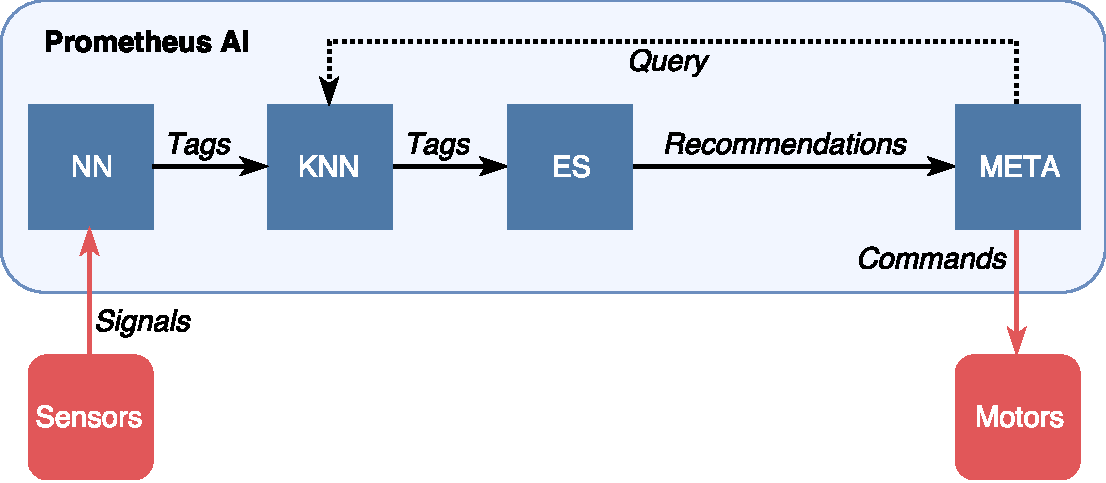
\includegraphics[width=\textwidth]{figures/ai_model_labeled.pdf}
	\caption{Prometheus AI model with labeled input and output.}
	\label{model_labeled}
\end{figure*}

\subsection{Summary}

With this full description of the Prometheus AI model, the system with labeled input and output can be seen in \autoref{model_labeled}.

\section{Problem}
\label{sec:problem}
% In this section you should describe the problem or system you are addressing in detail. Describe the project requirements and constraints.

The main task for this thesis is to construct the KNN and ES in Java. The requirements are that these layers should contain basic versions of the functionality described in \autoref{sec:background}. Another important task is to supervise the work of other undergraduate students working on Prometheus and to put systems in place to ensure a certain standard for the code. The design criteria for both these tasks will be discussed in \autoref{sec:design}, and their implementation will be discussed in \cref{sec:implementation}.

\section{Design}
\label{sec:design}
% In this section you must describe any design work that was already completed. Discuss any design decisions that have been made, and describe the process that was followed to make these decisions. Also discuss any results that have already been obtained this semester.

\subsection{Efficiency}
A very important consideration when designing the system is speed. Since the robots may have to react very quickly to stimuli in the environment, the reasoning in the AI must be as fast as possible. This is especially true in the hazardous environments for which this system could be useful for, as specified in \autoref{sec:intro}.

\subsection{Object Oriented Programming}
Another important design choice is to leverage object-oriented programming (OOP) as much as possible. OOP allows extensive planning before even beginning to write code, which can identify any flaws in the initial design. It also allows the code to be very clean and reusable \cite{oop}. Since Java is the programming language chosen for the project, OOP is also the natural way to proceed.  OOP principles such as polymorphism and encapsulation will be followed closely. One important OOP principle to use is abstraction. Indeed, the system should be as abstract as possible, while still performing its desired task. For instance, the system should be general enough to perform under simulations, as well as in real-life environments. It should also ideally be able to perform in vastly different environments, with varying tasks. Encapsulation can also be very useful, since each layer of the system has unique, localized functionality that does not need to be visible from the rest of the system.
\todo{Talk about more complex principles (Liskov, dependency inversion, injection, SOLID)}

\subsection{Readability \& Documentation}
One final design criterion is that the code written should be very easy to understand. This means implementing each method and class in the most intuitive way possible and providing good documentation to support the code. This is to ensure that anyone wanting to work with the code or looking to understand how the system works has an easy time doing so.

\subsection{Testing}
An important criterion is that the code be heavily tested. This includes integration tests, covering end-to-end functionality, and unit tests. The unit tests should be behavior-driven, so that a developer reading the tests can easily understand the purpose of the element being tested. The aim is that at least \SI{95}{percent} of the code be covered by tests.

\subsection{Quality Assurance}
With the numerous undergraduate students showing interest in working on Prometheus, there must be a system in place to ensure the quality of the code is upheld. This may include automatic testing of the code, as well as human review of code before being committed.

\section{Implementation}
\label{sec:implementation}

\subsection{Tags}

As described in \autoref{sec:background}, the entire system revolves around tags passed from layer to layer. For this reason, a lot of thought was put into the proper design of these tags.

The tags need to be as general as possible. A natural choice for this structure would be a Java \code{String}, which would be relatively simple to pass around the system. However, these tags represent various concepts; each tag can either be a fact, a recommendation or a rule. If implemented as \code{Strings}, the tags would have to be encoded on creation to represent each concept and decoded on use to retrieve the important information. This seems like a bad use of the OOP principles of Java. Furthermore, if specific functionality is needed in the future for each tag type, that can easily be implemented with a Java class. For these reasons, the tags are implemented using a \code{Tag} Java class, with \code{Predicate} and \code{Rule} subclasses. The \code{Predicate} class is a superclass of the \code{Fact} and \code{Recommendation} classes, as shown in \cref{fig:uml_tags}. This is a good example of using the inheritance principle of OOP. This should also make manipulating the Tags faster, while incurring a slight memory overhead. To store these Tags in a database, they can be converted to JSON format. On read from the database, they can be easily decoded. All these classes are present in the \code{tags} package of the code.

\begin{figure}[!htb]
	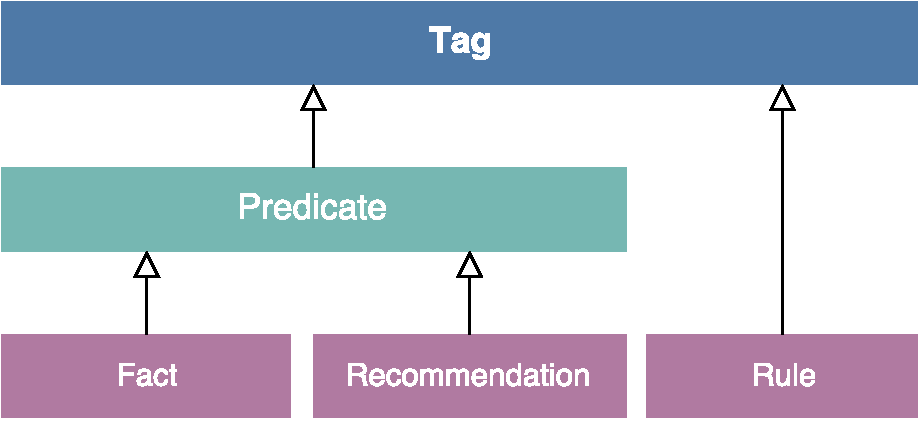
\includegraphics[width=\columnwidth]{figures/uml_tags.pdf}
	\caption{UML diagram of the major classes in the \code{tags} package.}
	\label{fig:uml_tags}
\end{figure}

The \code{Tag} and \code{Predicate} classes themselves are abstract. This means that an object may not be directly instantiated as either, but must be instantiated as one of its subclasses. This makes sense, since a tag \emph{must} be one of the three types: rule, recommendation or fact. This is an example of using the abstraction principle of OOP.

The \code{Rule} class has the following important fields:

\begin{labeling}{\code{outputPredicates}}
	\item[\code{inputFacts}] \code{Set} of input \code{Facts}.
	\item[\code{outputPredicates}] \code{Set} of output \code{Predicates}.
\end{labeling}

\subsection{Knowledge Node Network}

All code relating directly to the KNN was placed in the \code{knn} package of the project. A UML diagram of the important classes in the \code{knn} package can be seen in \cref{fig:uml_knn}.

\begin{figure}[!htb]
	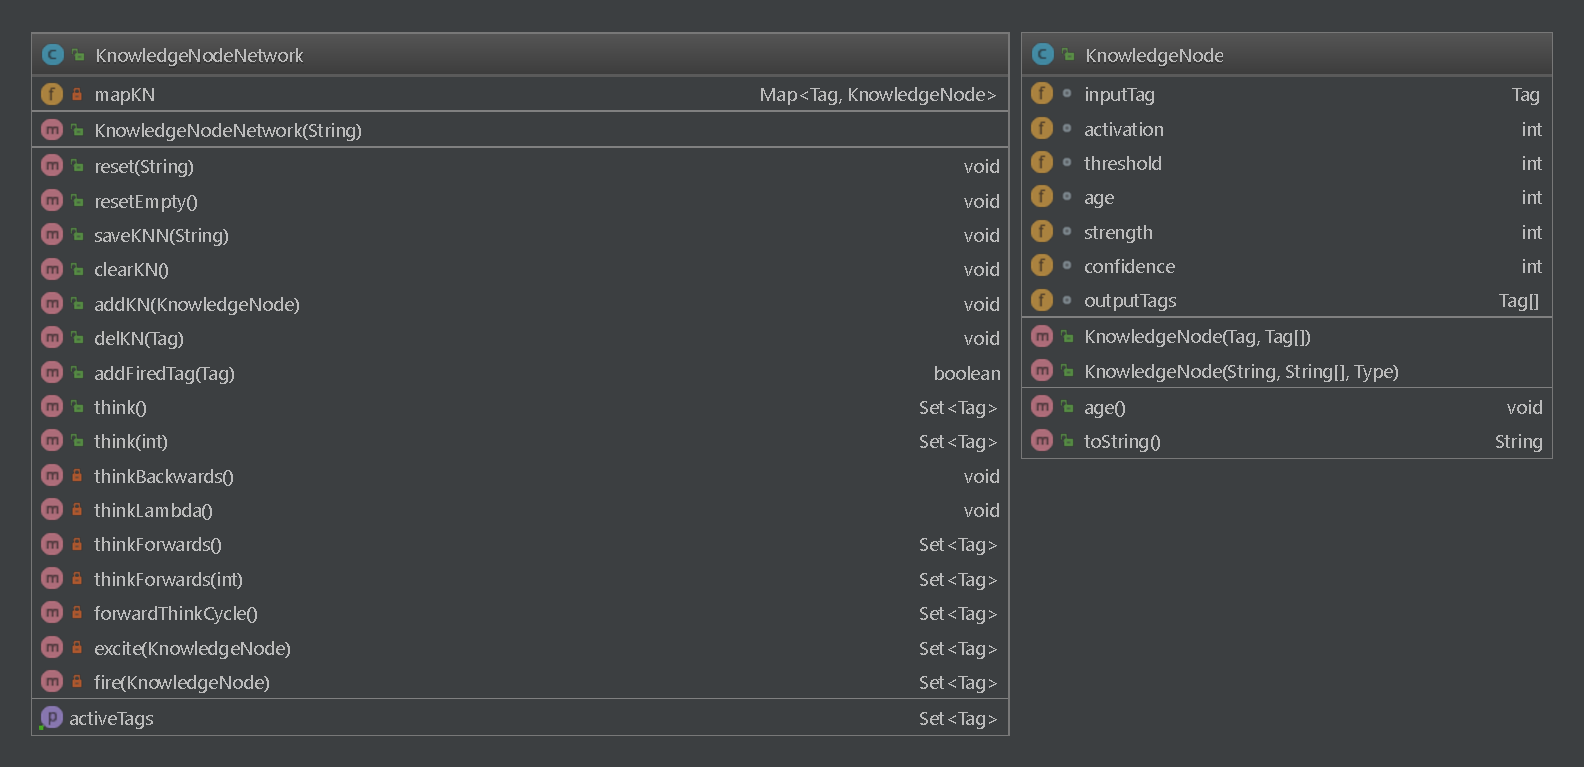
\includegraphics[width=\columnwidth]{figures/uml_knn.pdf}
	\caption{UML diagram of the major classes in the \code{knn} package.}
	\label{fig:uml_knn}
\end{figure}

The KNN layer is based around the \code{KnowledgeNodeNetwork} interface. Its implementation, \code{KnowledgeNodeNetworkImpl}, has the following fields:

\begin{labeling}{\code{activeTags}}
	\item[\code{mapKN}] One-to-one \code{HashMap} of input \code{Tag}s to associated \code{KnowledgeNode}s.
	\item[\code{activeTags}] \code{HashSet} of active \code{Tag}s, corresponding to input \code{Tag}s of fired \code{KnowledgeNode}s.
\end{labeling}

The choice of \code{HashSet} for the \code{activeTags} field is not arbitrary. Indeed, \code{HashSets} were used for most of the collections with variable size in the ES and KNN. The original specifications mentioned using \code{ArrayLists}, but, since there is no specific iteration order necessary for most operations in the ES and KNN, these collections were changed to \code{HashSets}. \code{HashSets} are also faster because they have $O(1)$ access time, whereas \code{ArrayLists} have $O(N)$, where $N$ is the number of elements in the collection. Access time is important because the tags in the KNN and ES are accessed often. \code{HashSets} also have the advantage of only permitting unique elements. This is useful because there should never be two copies of the same tag or the same KN in the system.

The \code{KnowledgeNode} class implements the functionality of a KN, which has the following important fields to implement the functionality described in \autoref{sec:background}:

\begin{labeling}{\code{outputTags}}
	\item[\code{inputTag}] Input \code{Tag}.
	\item[\code{outputTags}] \code{Array} of output \code{Tags}.
	\item[\code{activation}] \code{int} starting at 0, incrementing when the \code{KnowledgeNode} is excited.
	\item[\code{threshold}] \code{int} threshold that causes firing of the \code{KnowledgeNode}.
	\item[\code{strength}] \code{int} that biases the activation of a \code{KnowledgeNode}, causing early firing. The \code{KnowledgeNode} is fired if \code{(activation $\cdot$ strength) $\geq$ threshold}.
	\item[\code{confidence}] \code{int} representing the belief that the \code{inputTag} is true (0 to 100).
	\item[\code{age}] \code{int} representing the age of the \code{KnowledgeNode}.
\end{labeling}

The most important methods in the \code{KnowledgeNodeNetwork} are the ones relating to searching and thinking, as described in \cref{sec:background}. The search methods are \code{directSearch()}, \code{forwardSearch()}, \code{backwardSearch()} and \code{lambdaSearch()}. The \code{directSearch()} method takes as input the \code{Tag} to activate and returns the \code{Set} of \code{Tag}s activated as a result of exciting the \code{KnowledgeNode} associated with the input \code{Tag}. Note that the input \code{Tag} itself is not returned.
Similarly, the other search methods take a \code{Set} of \code{Tag}s as input and return the \code{Set} of \code{Tag}s activated as a result of searching. The other search methods also take a \code{ply} parameter specifying the depth of the search. If \code{ply} is 0, the search continues until quiescence, i.e., until no \code{Tag}s are activated during a search cycle.

For each of the search methods, there is an associated searcher class, i.e., \code{DirectSearcher}, \code{ForwardSearcher}, \code{BackwardSearcher} and \code{LambdaSearcher}. Delegating the search behavior to different classes allows for modularity and easy unit testing. Re-use of these classes was also taken advantage of, with \code{ForwardSearcher} using \code{DirectSearcher}, and \code{LambdaSearcher} using \code{ForwardSearcher} and \code{BackwardSearcher}, as shown in \cref{fig:uml_knn}. The \code{ForwardSearcher}, \code{BackwardSearcher} and \code{LambdaSearcher} also extend a \code{Searcher} abstract class, which handles some common functionality, i.e., searching until quiescence when the \code{ply} is 0.

Similarly, there are methods relating to thinking, i.e, \code{forwardThink()}, \code{backwardThink()} and \code{lambdaThink()}. These behave in the same way as their searching counterparts, except that they take as input all the currently active tags in the KNN, instead of user-provided input.
\todo{Talk about age implementation, design decisions.}

\subsection{Expert System}

All code relating directly to the ES was placed in the \code{es} package of the project. A UML diagram of the \code{es} package can be seen in \cref{fig:uml_es}.

\begin{figure}[!htb]
	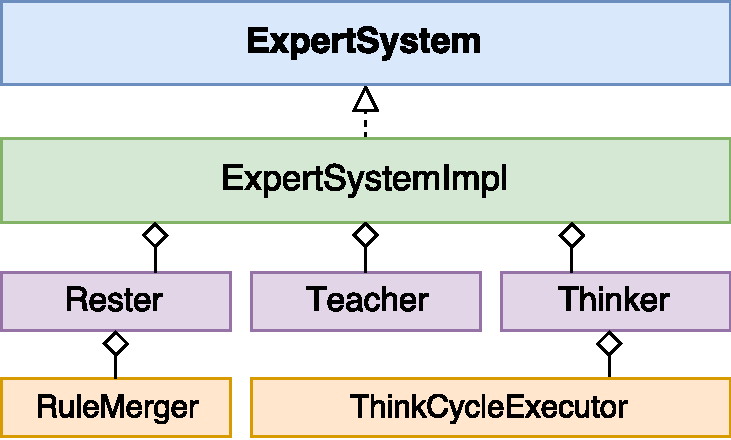
\includegraphics[width=\columnwidth]{figures/uml_es.pdf}
	\caption{UML diagram of the major classes in the \code{es} package.}
	\label{fig:uml_es}
\end{figure}

The ES layer is based around the \code{ExpertSystem} interface. Its implementation, \code{ExpertSystemImpl}, has the following important fields:

\begin{labeling}{\code{recommendations}}
	\item[\code{readyRules}] \code{HashSet} of \code{Rules} that have not been activated yet.
	\item[\code{activeRules}] \code{HashSet} of active \code{Rules}.
	\item[\code{facts}] \code{HashSet} of active \code{Facts}.
	\item[\code{recommendations}] \code{HashSet} of active \code{Recommendations}.
\end{labeling}

The most important method in the \code{ExpertSystem} is \code{think()}, which implements the functionality described in \cref{sec:background}. It has the following parameters:

\begin{labeling}{\code{generateRule}}
	\item[\code{ply}] The amount of thinking cycles to execute.
	\item[\code{generateRule}] If \code{true}, generates a \code{Rule} based on the active \code{Fact}s and the ones activated as a result of thinking.
\end{labeling}

The \code{think()} method has an associated \code{Thinker} class, whose sole purpose is to execute thinking cycles.

\subsection{Visualization}
The Java graph visualization library GraphStream was used to visualize the KNN and the process of searching or thinking through it. The graphing code created was placed in the \code{graphing} package. A UML diagram of the important classes in the \code{graphing} package can be seen in \cref{fig:uml_graphing}. A legend for reading the produced graph can be seen in \cref{fig:knn_graph_legend}.

\begin{figure}[!htb]
	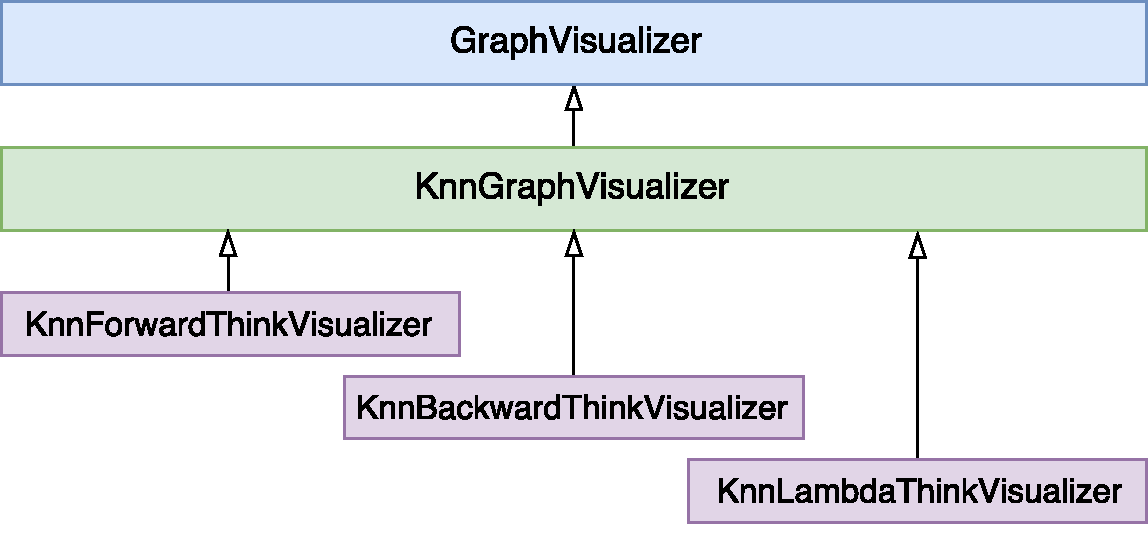
\includegraphics[width=\columnwidth]{figures/uml_graphing.pdf}
	{UML diagram of the important classes in the \code{graphing} package.}
	\label{fig:uml_graphing}
\end{figure}

\begin{figure*}[!htb]
	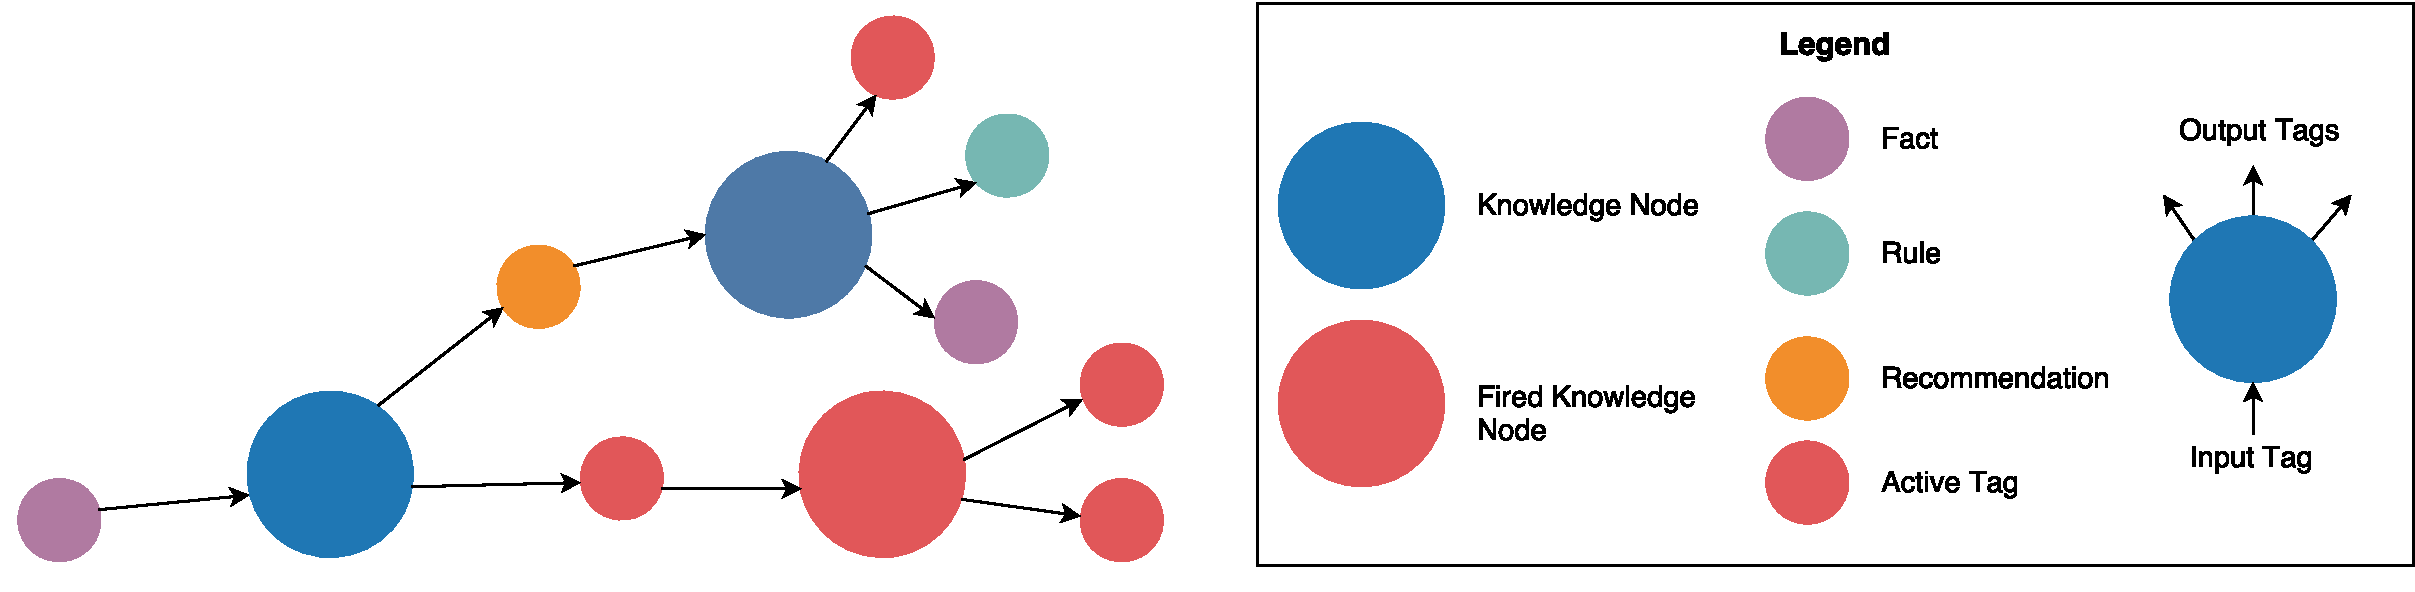
\includegraphics[width=\textwidth]{figures/knn_graph_legend.pdf}
	\caption{Legend for reading the graph produced by \code{KnnGraphVisualizer}.}
	\label{fig:knn_graph_legend}
\end{figure*}

\subsection{Documentation}
Extensive documentation was created in Javadoc\footnote{The Javadoc can be found here: \url{http://seanstappas.me/prometheus-ai/}}. Instructions are also provided on the README of the GitHub repository hosting the code\footnote{The GitHub repository can be found here: \url{https://github.com/seanstappas/prometheus-ai/}}.

\begin{figure*}[!htb]
	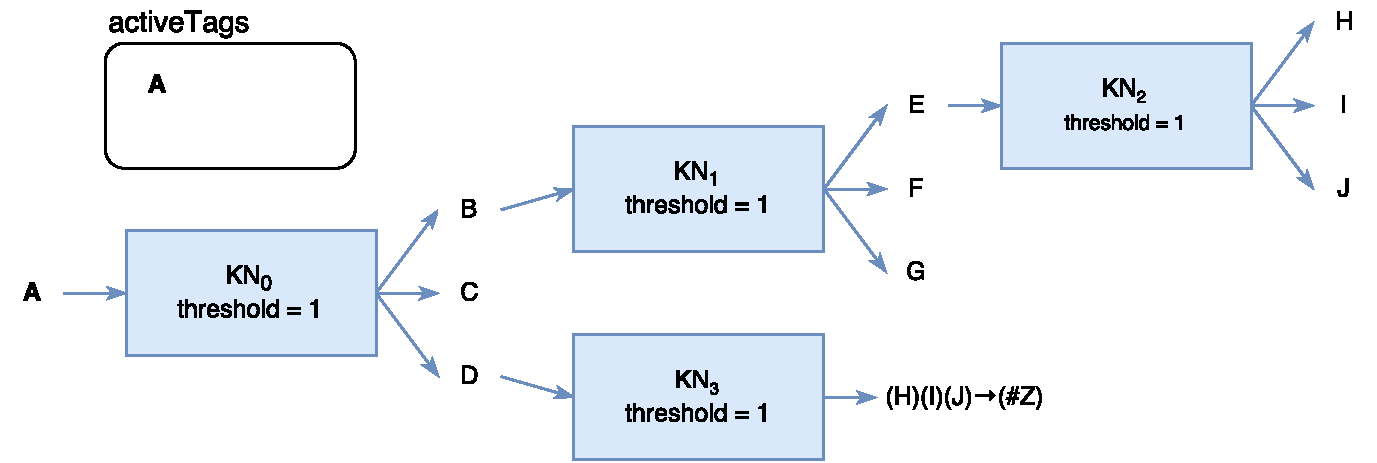
\includegraphics[width=\textwidth]{figures/testKNN.pdf}
	\caption[Setup for the \code{testKNN()} method.]
	{Initial setup for the \code{testKNN()} method.}
	\label{testKNN}
\end{figure*}

\begin{table*}[!htb]
	\large
	\centering
	\caption[Test setup for \code{testES()}.]
	{Test setup for \code{testES()}. Middle activation steps omitted.}
	\begin{tabular}{c | c | c | c | c} 
		\textbf{State} & \textbf{Ready Rules} & \textbf{Active Rules} & \specialcell{\textbf{Active} \\ \textbf{Facts}} & \specialcell{\textbf{Active} \\ \textbf{Recommendations}}  \\ \hline
		
		Initial & \specialcell{$(A)(B)\rightarrow(D)$ \\ $(D)(B)\rightarrow(E)$ \\ $(D)(E)\rightarrow(F)$\\ $(G)(A)\rightarrow(H)$ \\ $(E)(F)\rightarrow(\#Z)$} &  & $(A),(B)$ & $(\#X),(\#Y)$ \\ \hline
		
		$\vdots$ & $\vdots$ & $\vdots$ & $\vdots$ & $\vdots$ \\ \hline
		
		Final & $(G)(A)\rightarrow(H)$ & \specialcell{$(A)(B)\rightarrow(D)$ \\ $(D)(B)\rightarrow(E)$ \\ $(D)(E)\rightarrow(F)$ \\ $(E)(F)\rightarrow(\#Z)$} & \specialcell{$(A),(B),$ \\ $(D),(E)$ \\ $(F)$} & $(\#X),(\#Y),(\#Z)$		
	\end{tabular}
	\label{testES}
\end{table*}

\begin{table*}[!htb]
	\large
	\centering
	\caption{Test setup and activation for the ES portion of \code{testKNNandES()}.}
	\begin{tabular}{c | c | c | c | c} 
		\textbf{State} & \textbf{Ready Rules} & \textbf{Active Rules} & \specialcell{\textbf{Active} \\ \textbf{Facts}} & \specialcell{\textbf{Active} \\ \textbf{Recommendations}}  \\ \hline
		Initial
		&$(H)(I)(J)\rightarrow(\#Z)$
		& 
		& \specialcell{$(B),(C),(D)$ \\ $(E),(F),(G)$ \\ $(H),(I),(J)$}
		& \\ \hline
		
		Final
		&
		& $(H)(I)(J)\rightarrow(\#Z)$
		& \specialcell{$(B),(C),(D)$ \\ $(E),(F),(G)$ \\ $(H),(I),(J)$}
		& $(\#Z)$
	\end{tabular}
	\label{testKNNandES}
\end{table*}

\section{Results \& Tests} \label{sec:results}
\todo{BDD with Mockito + TestNG + Guice}
All tests on the system were conducted using the TestNG framework in Java, which provides a simple and intuitive way to create assertions in tests. These tests were placed in the \code{test} package of the project. A UML diagram of the \code{test} package can be seen in \autoref{uml_test} of the Appendix. The primary methods of interest in the test package are \code{testKNN()}, \code{testES()}, and \code{testKNNandES()}.

The test setup for the \code{testKNN()} method can be seen in \autoref{testKNN}. It creates a KNN, with every node having a \code{threshold} value of 1 to simplify the activation process. The system starts out with $A$ as the only active \code{Tag}, and \code{testKNN()} will make the KNN \code{think()} until natural quiescence. It is therefore expected that all the \code{Tags} shown in \autoref{testKNN} will become active by the end of the thinking process. The initial and final states are both asserted with TestNG in \code{testKNN()}, with positive results.

The test setup for the \code{testES()} method can be seen in \autoref{testES}. The columns from left to right (ignoring State) correspond to the elements in \code{readyRules}, \code{activeRules}, \code{facts}, and \code{recommendations}, respectively. The first row corresponds to the initial setup of the ES, and the last row corresponds to the expected final state. Both the initial and final states are asserted with TestNG in \code{testES()}, with positive results.

The \code{testKNNandES()} method has the same setup as \code{testKNN()} in \autoref{testKNN}, except the output active Tags from the KNN are passed on to the ES. The resulting setup and activation in the ES can be seen in \autoref{testKNNandES}. The initial and final states were also tested with TestNG with positive results.

\section{Impact on Society and the Environment}
\label{sec:impact}
% In one or two pages, discuss the environmental and/or social impact of your project. Your analysis should include your work at McGill as part of this project, however, the main focus should be on the product/system you are designing (e.g., the cost/benefit/risk of manufacturing it, the cost/benefit/risk for consumers using it) or the problem your thesis is addressing (e.g., how will solving the problem influence/affect/benefit society and the environment). Particular emphasis should be given to:


\subsection{Use of Non-renewable Resources}
% Consider all stages of the product from design, manufacturing, distribution, use by consumers, and disposal/recycling.

As purely a software project, there are no physical materials needed to construct this system. For this reason, less emphasis will be put on this section. The only related physical resources potentially needed are the materials needed to construct the robots and the computers to house the software. One area of concern could be the energy source of the robots themselves, which would probably vary depending on context. Ideally, the source should be a renewable one. For example, solar panels could be placed on the robots to provide energy.

\subsection{Environmental Benefits}
% Benefits to the environment, comparisons with more polluting technologies etc.

Prometheus could be used in a context beneficial to the environment. For example, the system could be used as a tool to control robots after oil spills, where the robots could theoretically contain the problem faster than humans and thus limit the risk on the environment. There is already research being done on employing robots in this context. Indeed, MIT's Senseable City Lab has been working on Seaswarm, a system composed of a fleet of vehicles to help clean future oil spills \cite{seaswarm}. An AI like Prometheus to control a swarm of robots like this could be very valuable. 

\subsection{Safety and Risk}
% To you undertaking the project, as well as to any potential users of the solution once it is finished.

It is critical that, once this system is completed, it is used in an ethical way, and for the right purposes. One example of use that may cause ethical concern is in a military setting, where an AI system like the one described here could be used in a battlefield in place of soldiers. Indeed, the US Department of Defense has plans to employ AI for autonomous weapons to attack targets without human intervention in the future \cite{military}. This would have the advantage of potentially saving human soldiers' lives \cite{define_military_ai}. However, there are also concerns because this would make it much easier to start a battle. More than 3000 AI and robotics researchers have signed an open letter arguing against a military AI arms race \cite{openletter}. They argue that autonomous weapons would not be beneficial to society, since they would be ideal for assassinations, destabilizing countries or selectively subduing or killing a population.

Another possible issue is the future loss of jobs to be done by humans, with automated systems like Prometheus replacing physical labour. This problem can be solved as a society, perhaps by having more support for universal basic income (UBI). Telsa CEO Elon Musk is a proponent of the idea, saying that UBI will be necessary in the future \cite{musk}. Microsoft co-founder Bill Gates suggests possibly having a tax on robots to help pay for this income \cite{gates}.

In the very long term, there are concerns with the possibility that an AI system might achieve intelligence and awareness close to a human. If such an AI were to obtain ``consciousness'' in its own way, should that entity be entitled to its own rights, like humans or animals are? The issue has been mentioned by the Institute for the Future, calling for the possibility of ``robo-rights'' in the future \cite{robo_rights}.


\subsection{Benefits to Society}
% Quality of life, economic benefits, etc.

This type of system could be extremely useful in many contexts in society. For instance, the system could be used to send and control robots in an area that would otherwise be very dangerous for humans. For example, robots are often used in the aftermath of nuclear disasters to prevent the unnecessary loss of human life. Indeed, even in the Chernobyl nuclear disaster, the Soviet authorities employed the use of robots to avoid losses of human life \cite{chernobyl}. With an AI like Prometheus, the robots could be controlled in an intelligent manner.

The system could also be used to further space exploration, with an AI controlling multiple robots exploring the surface of Mars, for instance. The value of AI in this context has been clearly shown, with the Mars Curiosity rover recently being upgraded to have its own AI system using computer vision to identify rocks \cite{rover}. This system can therefore help further important cutting-edge research in space exploration.

\section{Conclusion}
% Use this section to summarize what was accomplished in this semester, provide a summary of the next steps and share any insight you have learned.

This semester, prototypes of the Expert System (ES) and Knowledge Node Network (KNN) layers of the Prometheus AI model were completed in Java based on personal design criteria and feedback from the supervisor. The design of the prototypes has required a great deal of thought and planning to ensure efficiency and proper behaviour. These prototypes were tested using the TestNG Java framework with positive results, and extensive Javadoc was produced. Possible impacts on the environment and society were also discussed.

The main goal for next semester is to finalize the entire system, implementing more complex features that were omitted for this prototype stage. This will also require proper integration between the work done in this report (KNN and ES), and outside this report (NN and META). Finally, the entire system will have to be tested, in simulation and with physical robots.

\clearpage
\onecolumn
\appendix

\renewcommand\thefigure{\thesection.\arabic{figure}}
\setcounter{figure}{0}    

\section{UML Diagrams}
\label{sec:uml}

%\begin{figure}[!htb]
%	\centering
%	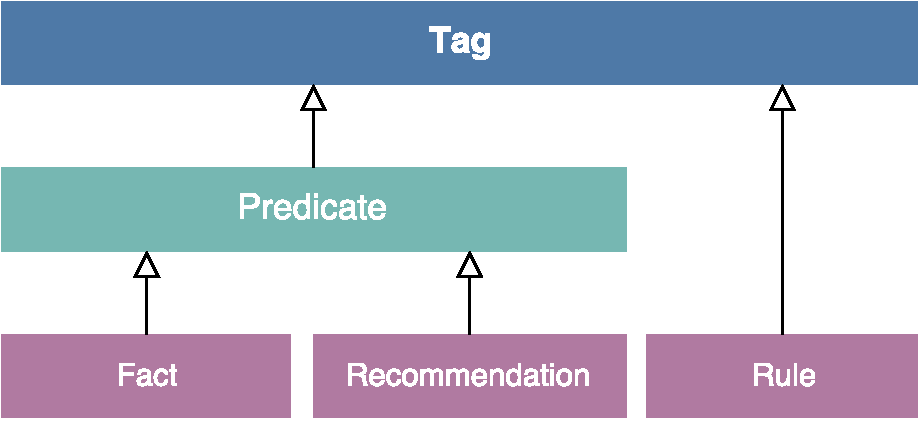
\includegraphics[width=\columnwidth]{figures/uml_tags.pdf}
%	\caption{UML diagram of the \code{tags} package.}
%	\label{uml_tags}
%\end{figure}

\missingfigure{UML Diagrams of ES and KNN packages}

\missingfigure{Guice dependency graph diagram}

\clearpage

\bibliography{readings}{}
\bibliographystyle{IEEEtran}

\end{document}